%%%%%%%%%%%%%%%%%%%%%%%%%%%%%%%%%%%%%%%%%
% Dreuw & Deselaer's Poster
% LaTeX Template
% Version 1.0 (11/04/13)
%
% Created by:
% Philippe Dreuw and Thomas Deselaers
% http://www-i6.informatik.rwth-aachen.de/~dreuw/latexbeamerposter.php
%
% This template has been downloaded from:
% http://www.LaTeXTemplates.com
%
% License:
% CC BY-NC-SA 3.0 (http://creativecommons.org/licenses/by-nc-sa/3.0/)
%
%%%%%%%%%%%%%%%%%%%%%%%%%%%%%%%%%%%%%%%%%

%----------------------------------------------------------------------------------------
%	PACKAGES AND OTHER DOCUMENT CONFIGURATIONS
%----------------------------------------------------------------------------------------

\documentclass[final,hyperref={pdfpagelabels=false}]{beamer}

\usepackage[orientation=portrait,size=a4,scale=1.3]{beamerposter} % Use the beamerposter package for laying out the poster with a portrait orientation and an a0 paper size

\usetheme{I6pd2} % Use the I6pd2 theme supplied with this template

\usepackage[english]{babel} % English language/hyphenation

\usepackage{amsmath,amsthm,amssymb,latexsym} % For including math equations, theorems, symbols, etc

%\usepackage{times}\usefonttheme{professionalfonts}  % Uncomment to use Times as the main font
%\usefonttheme[onlymath]{serif} % Uncomment to use a Serif font within math environments

\boldmath % Use bold for everything within the math environment

\usepackage{booktabs} % Top and bottom rules for tables

\graphicspath{{figures/}} % Location of the graphics files

\usecaptiontemplate{\small\structure{\insertcaptionname~\insertcaptionnumber: }\insertcaption} % A fix for figure numbering

%----------------------------------------------------------------------------------------
%	TITLE SECTION 
%----------------------------------------------------------------------------------------

\title{\huge YOLOv7 Small Object Detection Optimization to Detect Airborne Objects} % Poster title

\author[Dion Solang]{ 
  \parbox[t]{7cm}{
    \textbf{Author}\\
    Dion Andreas Solang\\
    NRP 07211940000039
  }
  \parbox[t]{7cm}{
    \textbf{Advisors}\\
    Reza Fuad Rachmadi, S.T., M.T., Ph.D\\
    Dr. I Ketut Eddy Purnama S.T., M.T.
  }
} % Author(s)

\institute{
  Department of Computer Engineering\\
  Institut Teknologi Sepuluh Nopember} % Institution(s)

%----------------------------------------------------------------------------------------
%	FOOTER TEXT
%----------------------------------------------------------------------------------------

\newcommand{\leftfoot}{messier12.github.io/yolov7ta} % Left footer text

\newcommand{\rightfoot}{solang.dion@gmail.com} % Right footer text

%----------------------------------------------------------------------------------------

\begin{document}

\addtobeamertemplate{block end}{}{\vspace*{2ex}} % White space under blocks

\begin{frame}[t] % The whole poster is enclosed in one beamer frame

\begin{block}{ABSTRACT}
  Airborne objects appear very small on cameras.
  YOLOv7 is the state of the art real-time object detector optimized for general object detections.
  Thus, to detect airborne objects with YOLOv7, modifications are needed to be applied.
  The purpose of this research is to find a modification solution for YOLOv7 to optimize its small object detection capability especially for airborne objects.
  Modifications to be applied on YOLOv7 consists of architecture modifications and bag-of-freebies modifications.
  Architecture modifications consist of neck modification and head layer addition.
  Bag-of-freebies modifications consist of mosaic data augmentation dan active anchor recalculation.
  These modifications will be combined one with another and have their performance tested.
  Modifications that produces model with the highest mAP score on airborne objects dataset will be chosen as the optimization solution of this research.
\end{block}

\begin{columns}[t] % The whole poster consists of two major columns, each of which can be subdivided further with another \begin{columns} block - the [t] argument aligns each column's content to the top

\begin{column}{.02\textwidth}\end{column} % Empty spacer column

\begin{column}{.465\textwidth} % The first column

%----------------------------------------------------------------------------------------
%	OBJECTIVES
%----------------------------------------------------------------------------------------

\begin{block}{Objective}
  The objective of this research is to find modifications that can be made to YOLOv7
  such that it could detect airborne objects better.
\end{block}

%----------------------------------------------------------------------------------------
%	INTRODUCTION
%----------------------------------------------------------------------------------------
            
\begin{block}{Introduction}
  One of the greatest challenge in autonomous flight
  is about the problem of sensing and avoiding (SAA) airborne objects like bird, airplane, helicopter, and other.
  Camera is a popular choice of sensor for this task due to its cheaper price and small payload.
  One problem however, airborne objects appear very small on cameras.
  The size is about 4-1000 pixels in a 20 million pixels camera.
  Detecting such small objects is very challenging.

  In this study, we will try to optimize YOLOv7 to solve this challenge.
  YOLOv7 is an general real-time object detection architecture with the highest accuracy at the time its paper was published (July 2022).
  YOLOv7 can be scaled down so that it can run on edge computing devices such as Jetson TX2.
  Its high accuracy and low computational cost were the reason why YOLOv7 was chosen for this study.

  To optimize YOLOv7, we will carry out modifications to the bag-of-freebies and architecture of YOLOv7.
  These modifications however must not cause YOLOv7 lose its ability to detect objects in real-time.

\end{block}

%----------------------------------------------------------------------------------------
%	MATERIALS
%----------------------------------------------------------------------------------------

\begin{block}{Related Works}
  There are some similar attempts of modifying YOLO architecture to improve its object detection capability.
  \begin{itemize}
    \item YOLOZ
    \begin{itemize}
      \item Based on YOLOv5.
      \item Changed YOLOv5 backbone to DenseNet.
      \item Changed the neck to biFPN.
      \item Optimized to detect autonomous racing cones.
    \end{itemize}
    \item exYOLO
    \begin{itemize}
      \item Based on YOLOv3.
      \item Added Receptive Field Block prior to feature fusion in the neck.
    \end{itemize}
  \end{itemize}

\end{block}

\begin{block}{Methodology: Flow of Work}

\begin{figure}
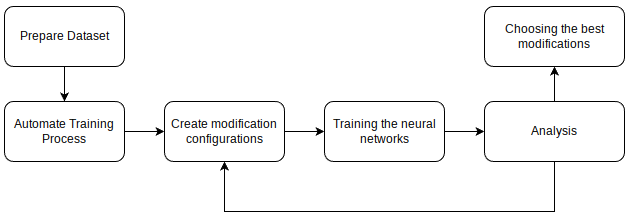
\includegraphics[width=\linewidth]{metodologi.png}
\end{figure}

\end{block}



%  %----------------------------------------------------------------------------------------
%  %	METHODS
%  %----------------------------------------------------------------------------------------
%  
%  \begin{block}{Methods}
%  
%  \begin{itemize}
%  \item Maecenas Vel Nisl Elit
%  \begin{itemize}
%  \item Suspendisse potenti. Fusce a est eget turpis rhoncus varius sed sed dui. Cras justo nibh, bibendum a cursus eget, consequat et dui. Maecenas vel nisl elit, sed dignissim dolor. 
%  \item In hac habitasse platea dictumst.
%  \end{itemize}
%  
%  \item Viewpoint Matching Constraints
%  \begin{itemize}
%  \item Cum sociis natoque penatibus et magnis dis parturient montes, nascetur ridiculus mus. 
%  \item Proin in nisi diam.
%  \item Nam ultricies pellentesque nunc, ultrices volutpat nisl ultrices a.
%  \end{itemize}
%  
%  \item Volutpat 
%  \begin{itemize}
%  \item Duis semper lorem eget dui dignissim porttitor.
%  \item Nulla facilisi. In ullamcorper lorem quis dolor.
%  \end{itemize}
%  \end{itemize}
%  
%  \end{block}
%  
%  %----------------------------------------------------------------------------------------
%  %	MATHEMATICAL SECTION
%  %----------------------------------------------------------------------------------------
%  
%  \begin{block}{Mathematical Section}
%  
%  \begin{itemize}
%  \item Maecenas Ultricies Feugiat Velit Non Mattis.
%  \begin{itemize}
%  \item Duis ante erat, bibendum nec tempus nec, interdum quis est. Nulla at mollis tortor. Phasellus quis leo dolor, aliquam laoreet orci $X$ Donec dapibus sagittis neque eu nec, interdum quis est. $Y_n, n=1,\cdots,N$ ndum nec tempus nec, interd
%  \begin{align*}
%  X \rightarrow r(X) & = \arg \max_{c} \Big\{ \max_n \big\{ \sum_{x_i \in X} \delta(x_i,Y_{n,c})\big\} \Big\} 
%  \end{align*}
%  \item Cras faucibus scelerisque cursus. Proin ut vestibulum augue. $\delta(x_i,Y_{n,c})$
%  \end{itemize}
%  \item Fusce tempus arcu id ligula varius dictum. Donec ut nisl dui, ac consectetur elit. In nec enim porta augue venenatis sollicitudin. Phasellus quis nunc neque. Suspendisse mauris diam, suscipit non gravida in, placerat id enim. Ut nec ipsum in lectus ultrices sagittis.
%  \end{itemize}
%  
%  \end{block}
%  
%  %----------------------------------------------------------------------------------------

\end{column} % End of the first column

\begin{column}{.03\textwidth}\end{column} % Empty spacer column
 
\begin{column}{.465\textwidth} % The second column

%----------------------------------------------------------------------------------------
%	RESULTS
%----------------------------------------------------------------------------------------
\begin{block}{Methodology: Step by Step}
  To conduct this study, first the dataset must be prepared to conform with format understandable by YOLOv7.
  Then, to aid and accelerate the process of this study, we will automate the training process.
  Modification configurations will be made and then inputted to the trainer. 
  These modifications might or might not include a combinations of modifications candidates.
  The trainer will built neural network according to the modification configuration and train them.
  The traned neural networks will be analyzed for their performance and to look for potential modifications that can be made to optimize the neural network more.
  If such modification was found, we will create a configuration for it and then feed it to the trainer.
  Finally, among all of the modifications, the best model will be chosen.
  The best model will be decided according to their mAP score.
\end{block}


\begin{block}{Modifications Candidates}
  \begin{itemize}
    \item Bag-of-Freebies Modifications
    \begin{itemize}
      \item On-training Anchor Box Recalculation
      A layer will be added in the neural network to learn the optimal size
      for anchor box. 
      In most YOLO architectures, the anchor box are constant and calculated prior to training.
      \item Mosaic Augmentation
      Mosaic Augmentations has been proven to increase the object detection accuracy in YOLOv4 and YOLOv5.
    \end{itemize}
    \item Architecture Modifications
    \begin{itemize}
      \item Neck Modifications
      Some layer of the neck will be modified to take input from a more shallow layer of the backbone of YOLOv7.
      \item Head layer addition
      Another head layer will be added so that YOLOv7 can detect on a higher scale.
    \end{itemize}
  \end{itemize}
\end{block}

\begin{block}{Sampled Dataset Distribution}

\begin{table}
\small
\begin{tabular}{|c|c|c|c|c|c|c|}
        \hline
        Division &Total & \multicolumn{4}{c}{Percentage}&\\
                           \cline{3-7}
                  &image& Airplane & Helicopter & Bird & \emph{Other} & Negative\\
        \hline
        Train  &54k &23,75\%  &23,75\%     &23,75\% &23,75\%       &5\%\\
        \hline                                              
        Valid&3k  &20\%     &20\%        &20\%    &20\%          &20\%\\
        \hline                                                           
        Test      &3k  &20\%     &20\%        &20\%    &20\%          &20\%\\
        \hline
\end{tabular}
%  \begin{tabular}{l l l}
%  \toprule
%  \textbf{Treatments} & \textbf{Response 1} & \textbf{Response 2}\\
%  \midrule
%  Treatment 1 & 0.0003262 & 0.562 \\
%  Treatment 2 & 0.0015681 & 0.910 \\
%  Treatment 3 & 0.0009271 & 0.296 \\
%  \bottomrule
%  \end{tabular}
\end{table}

\end{block}

%------------------------------------------------

% %----------------------------------------------------------------------------------------
% %	ACKNOWLEDGEMENTS
% %----------------------------------------------------------------------------------------
% 
% \begin{block}{Acknowledgments}
% 
% \begin{itemize}
% \item Nam mollis tristique neque eu luctus. Suspendisse rutrum congue nisi sed convallis. Aenean id neque dolor. Pellentesque habitant morbi tristique senectus et netus et malesuada fames ac turpis egestas.
% \end{itemize}
% 
% \end{block}
% 
% %----------------------------------------------------------------------------------------
% %	CONTACT INFORMATION
% %----------------------------------------------------------------------------------------
% 
\setbeamercolor{block title}{fg=black,bg=orange!70} % Change the block title color

\begin{block}{Contact Information}

\begin{itemize}
\item Implementation: \href{https://github.com/messier12/final-project-yolo-optimization.git}{https://github.com/messier12/final-project-yolo-optimization.git}
\item Email: \href{mailto:solang.dion@gmail.com}{solang.dion@gmail.com}
\item Phone: +62 813 2752 2023
\end{itemize}

\end{block}

%----------------------------------------------------------------------------------------

\end{column} % End of the second column

\begin{column}{.015\textwidth}\end{column} % Empty spacer column

\end{columns} % End of all the columns in the poster

\end{frame} % End of the enclosing frame

\end{document}